\documentclass[11pt]{article}
\usepackage[margin=0.86in]{geometry}
\usepackage{amsmath,amssymb,amsthm,booktabs,graphicx,microtype,xcolor}
\usepackage[hidelinks]{hyperref}
\setlength{\parindent}{0pt}
\setlength{\parskip}{0.5em}
\newtheorem{theorem}{Theorem}
\newtheorem{lemma}[theorem]{Lemma}
\newtheorem{corollary}[theorem]{Corollary}
\newcommand{\R}{\mathbb R}
\newcommand{\N}{\mathbb N_0}
\newcommand{\elltwo}{\ell^2(\N)}
\newcommand{\supp}{\operatorname{supp}}
\newcommand{\cstatus}{\textcolor{blue!60!black}{\textbf{candidate full solution---likely valid}}}

\begin{document}

\begin{center}
{\Large\bfseries Polynomially bounded solutions are dense in the Jacobi spectrum}\par
\vspace{0.35em}
{\large Closing the conjectured reverse inclusion in arXiv:1204.3322}\par
\vspace{0.45em}
\cstatus
\end{center}

\section*{1. Source question}

Dale T. Smith studies the self-adjoint half-line difference equation
\begin{equation}\label{eq:smith}
 -\Delta\!\left(a_{n-1}\Delta y_{n-1}\right)+b_ny_n=\lambda y_n,
 \qquad n=0,1,\ldots,
\end{equation}
where $a_{n-1}>0$, $b_n\in\R$, and every solution obeys the left boundary condition $y_{-1}=0$ \cite{Smith}.  Let $B$ be the associated operator on $\elltwo$.  Under the coefficient-growth and limit-point hypotheses displayed below, Smith's Theorem 2.3 proves
\[
 \overline E\subseteq\sigma(B),
 \qquad
 E=\{\lambda\in\R:\eqref{eq:smith}\text{ has a polynomially bounded solution}\}.
\]

\begin{center}
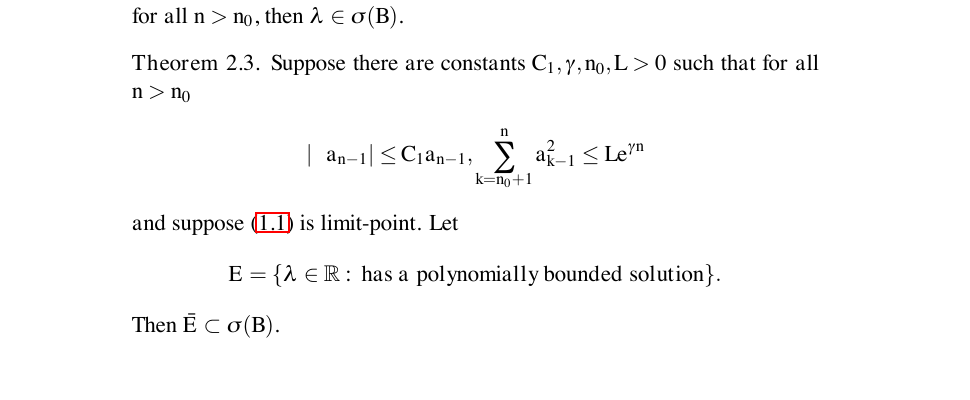
\includegraphics[width=0.88\textwidth]{figures/source_theorem_2_3.png}
\end{center}

On PDF page 11, Theorem 3.2 records a polynomial bound for the orthogonal-polynomial solution at spectral-measure almost every $\lambda$, but the paper then says that more is needed to prove the conjecture $\overline E=\sigma(B)$.

\begin{center}
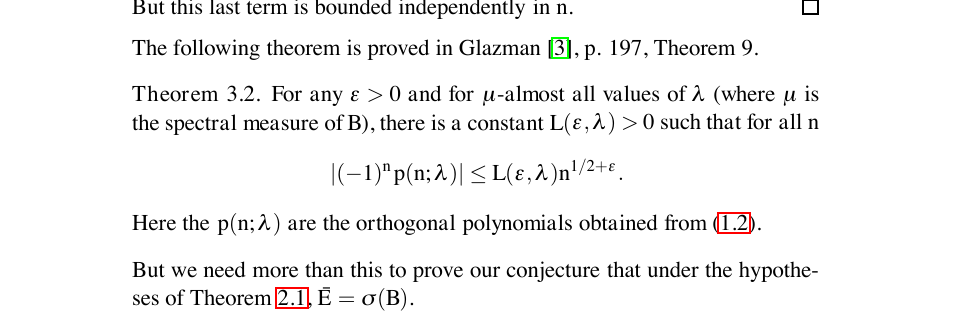
\includegraphics[width=0.88\textwidth]{figures/source_theorem_3_2_conjecture.png}
\end{center}

The extra ingredient is that this particular spectral measure has support equal to the whole spectrum.  That follows from cyclicity of the first Jacobi basis vector.

\section*{2. Exact statement}

Write $c_n=b_n+a_n+a_{n-1}$.  After the unitary sign change $y_n\mapsto(-1)^ny_n$, equation \eqref{eq:smith} becomes the Jacobi recurrence
\begin{equation}\label{eq:jacobi}
 a_np_{n+1}(\lambda)+c_np_n(\lambda)+a_{n-1}p_{n-1}(\lambda)
 =\lambda p_n(\lambda),
 \qquad p_{-1}=0,\quad p_0=1.
\end{equation}
Let $J$ be the corresponding Jacobi operator; it is unitarily equivalent to $B$ and the sign change fixes the first basis vector $e_0$.  In the limit-point case $J$ is self-adjoint.  Its scalar spectral measure at $e_0$ is the orthogonality measure $\mu$ for the polynomials $p_n$.

\begin{theorem}[Smith's conjecture]\label{thm:main}
Suppose that there are constants $C_1,\gamma,n_0,L>0$ such that, for every $n>n_0$,
\begin{equation}\label{eq:growth}
 |\Delta a_{n-1}|\le C_1a_{n-1},
 \qquad
 \sum_{k=n_0+1}^{n}a_{k-1}^2\le Le^{\gamma n},
\end{equation}
and suppose \eqref{eq:smith} is limit-point.  Then
\[
 \boxed{\ \overline E=\sigma(B)\ }.
\]
More precisely, for every $\varepsilon>0$, the set of $\lambda$ for which the canonical solution $(-1)^np_n(\lambda)$ satisfies
\[
 |p_n(\lambda)|\le C_{\lambda,\varepsilon}(n+1)^{1/2+\varepsilon}
 \quad(n\ge0)
\]
has full $\mu$-measure and is dense in $\sigma(B)$.
\end{theorem}

\section*{3. Proof intuition}

There are two logically independent halves.  Smith's Shnol-type theorem says that any polynomially bounded solution forces its parameter into the spectrum; this is where the growth assumptions \eqref{eq:growth} enter.

For the converse density, orthonormality gives $\int |p_n|^2\,d\mu=1$.  Weight these identities by the summable sequence $(n+1)^{-1-2\varepsilon}$ and apply Tonelli.  For $\mu$-almost every $\lambda$, all the values $p_n(\lambda)$ are then controlled by one finite weighted square sum, yielding the claimed polynomial bound.  Finally, $e_0$ is cyclic: the three-term recurrence generates every basis vector from $e_0$.  Hence $\supp\mu=\sigma(J)$.  A full-measure subset of a measure is dense in its support, which supplies exactly the missing inclusion.

\clearpage
\section*{4. The two spectral-measure lemmas}

\begin{lemma}[cyclicity and full support]\label{lem:cyclic}
Let $J$ be any self-adjoint half-line Jacobi operator whose off-diagonal coefficients $a_n$ are all nonzero, and let $\mu(S)=\langle E_J(S)e_0,e_0\rangle$.  Then $e_0$ is cyclic for $J$ and
\[
 \supp\mu=\sigma(J).
\]
\end{lemma}

\begin{proof}
Every finitely supported vector lies in the domain of the Jacobi expression.  From
\[
 Je_n=a_ne_{n+1}+c_ne_n+a_{n-1}e_{n-1}
\]
(with the $e_{-1}$ term absent) and $a_n\ne0$, induction gives a polynomial $q_n$ such that $e_n=q_n(J)e_0$.  Thus the cyclic subspace generated by $e_0$ contains every basis vector and is all of $\elltwo$.

The cyclic spectral theorem now represents $J$ as multiplication by $x$ on $L^2(\mu)$ and sends $e_0$ to the constant function $1$.  The spectrum of this multiplication operator is the closed topological support of $\mu$.  Therefore $\supp\mu=\sigma(J)$.
\end{proof}

\begin{lemma}[almost-everywhere polynomial bound]\label{lem:tonelli}
In the setting of Lemma \ref{lem:cyclic}, let $p_n$ be the normalized recurrence polynomials, so that
\[
 \int_{\R}|p_n(\lambda)|^2\,d\mu(\lambda)=1.
\]
For each $\varepsilon>0$, for $\mu$-almost every $\lambda$ there is a finite $C_{\lambda,\varepsilon}$ satisfying
\[
 |p_n(\lambda)|\le C_{\lambda,\varepsilon}(n+1)^{1/2+\varepsilon}
 \qquad(n\ge0).
\]
\end{lemma}

\begin{proof}
All summands are nonnegative, so Tonelli's theorem and orthonormality give
\begin{align*}
 \int_{\R}\sum_{n=0}^{\infty}
 \frac{|p_n(\lambda)|^2}{(n+1)^{1+2\varepsilon}}\,d\mu(\lambda)
 &=\sum_{n=0}^{\infty}\frac{1}{(n+1)^{1+2\varepsilon}}
 \int_{\R}|p_n(\lambda)|^2\,d\mu(\lambda)\\
 &=\sum_{n=0}^{\infty}\frac{1}{(n+1)^{1+2\varepsilon}}<\infty.
\end{align*}
Consequently, for $\mu$-almost every $\lambda$ the pointwise series has a finite value $S_\varepsilon(\lambda)$.  Each one of its terms is at most that value, and hence
\[
 |p_n(\lambda)|
 \le \sqrt{S_\varepsilon(\lambda)}(n+1)^{1/2+\varepsilon}.
\]
Take $C_{\lambda,\varepsilon}=\sqrt{S_\varepsilon(\lambda)}$.
\end{proof}

\clearpage
\section*{5. Proof of Theorem \ref{thm:main}}

Fix one $\varepsilon>0$ and let $G_\varepsilon$ be the full-$\mu$-measure set supplied by Lemma \ref{lem:tonelli}.  For every $\lambda\in G_\varepsilon$, the sequence $(-1)^np_n(\lambda)$ solves Smith's original equation \eqref{eq:smith} and is polynomially bounded.  Thus
\[
 G_\varepsilon\subseteq E,
 \qquad \mu(\R\setminus E)=0.
\]

We claim that $\sigma(B)\subseteq\overline E$.  Since $B$ and $J$ are unitarily equivalent and $e_0$ is unchanged, Lemma \ref{lem:cyclic} gives
\[
 \sigma(B)=\sigma(J)=\supp\mu.
\]
If $\lambda_0\in\sigma(B)$ and $U$ is any open neighborhood of $\lambda_0$, then $\mu(U)>0$ by the definition of support.  Because $E$ has full $\mu$-measure, $\mu(U\cap E)=\mu(U)>0$, so $U\cap E\ne\varnothing$.  Hence $\lambda_0\in\overline E$.

Conversely, Smith's Theorem 2.3 applies under \eqref{eq:growth} and the limit-point assumption and gives $\overline E\subseteq\sigma(B)$ \cite{Smith}.  Combining the two inclusions proves the equality.  The same argument works for every fixed $\varepsilon>0$, proving the final assertion.

\section*{6. Stronger density half and edge cases}

\begin{corollary}[growth-free converse-Shnol density]\label{cor:stronger}
For every self-adjoint half-line Jacobi operator with nonzero off-diagonal coefficients, and every $\varepsilon>0$, the parameters whose canonical generalized eigenfunction is $O((n+1)^{1/2+\varepsilon})$ form a full-spectral-measure subset dense in the spectrum.
\end{corollary}

This is precisely Lemmas \ref{lem:cyclic} and \ref{lem:tonelli}; no coefficient-growth assumption is used.

\emph{Eigenvalues and singular spectrum.}  Atoms cause no problem, and no absolute continuity is used: every neighborhood of every support point has positive measure.

\emph{Unbounded spectrum.}  The density argument is local and uses only finite open neighborhoods.

\emph{Constants and boundary data.}  The constant $C_{\lambda,\varepsilon}$ may depend on $\lambda$; no uniform bound is claimed.  Also $p_{-1}=0,p_0=1$, so $(-1)^np_n$ is an admissible nonzero solution of the source equation.

\emph{Limit-circle scope.}  A chosen self-adjoint Jacobi extension can still have a cyclic scalar measure, but Smith's reverse inclusion is not available as stated.  No equality for such extensions is claimed here.

\section*{7. Verification and novelty boundary}

The only external mathematical input in the new inclusion is the standard cyclic spectral theorem; the cyclicity and Tonelli estimates are proved above.  The other inclusion is exactly Smith's Theorem 2.3.  The proof was stress-tested at the domain/cyclicity induction, identification of the orthogonality measure with the scalar spectral measure, support versus spectrum, the almost-everywhere quantifier, and passage from full measure to density.

A bounded novelty search used the run's exact-id and keyword indexes.  It also covered the arXiv record and citation trail for 1204.3322, plus web searches combining the title, author, ``polynomially bounded solution,'' ``closure $E$,'' Jacobi, Shnol, spectral measure, and generalized eigenfunction terminology.  It found broad converse-Shnol and generalized-eigenfunction results, but no later paper explicitly resolving this exact conjecture.  This is not a publication-level priority search.

There is an important provenance caveat.  The downloadable TeX source of 1204.3322 contains a commented-out short proof sketch aimed at the same conclusion, although the rendered paper omits it and explicitly retains the statement as a conjecture.  That sketch invokes positive spectral measure in a missing open part of the spectrum without recording why the chosen measure has full support.  Lemma \ref{lem:cyclic} supplies that bridge, while Lemma \ref{lem:tonelli} makes the almost-everywhere estimate self-contained.  Accordingly, confidence in validity is high, but novelty confidence is low.

\textbf{Mathematical-validity confidence: 97/100.}  Recommended human review: verify the scalar spectral-measure identification and the source hypotheses of Theorem 2.3 first; then check whether the commented source sketch or an older Jacobi/converse-Shnol reference should receive priority credit.

\begin{thebibliography}{9}
\bibitem{Smith}
D.~T.~Smith,
\emph{Spectral Analysis of a Class of Self-Adjoint Difference Equations},
arXiv:1204.3322 (2012).

\bibitem{Teschl}
G.~Teschl,
\emph{Jacobi Operators and Completely Integrable Nonlinear Lattices},
Mathematical Surveys and Monographs 72, American Mathematical Society, 2000.
\end{thebibliography}

\end{document}
